\chapter{梯级系统性能评估}
\section{系统简介}

第\ref{sec:sst}节选出了两种典型的梯级系统拓扑结构用于研究工作。需要指出的是,第\ref{cha:osgs}章提出并分析了分段加热系统。分段加热系统比传统的蒸汽发生系统具有更好的热效率和㶲效率。然而,本章的梯级系统并没有使用改分段加热系统,这是因为,首先,为了更加清晰地表明本文所提出的梯级系统因梯级集热和梯级利用带来的收益,本章的梯级系统不使用分段加热系统。其次,同使用传统的蒸汽发生系统的太阳能光热发电系统相比,使用分段加热系统的太阳能光热发电系统只是改变了太阳能场部分。因此可以方便地将分段加热系统引入梯级系统而不影响其它部分的计算。最后,第\ref{cha:osgs}章提出的分段加热系统有很大的改进空间,值得以后进行更深入地研究。

第\ref{sec:sst}节选出了两种典型的梯级系统拓扑结构都采用了多种型式的集热器和多个热力循环来实现能量的梯级收集和梯级利用。然而,本章主要研究第一个拓扑结构,因为它使用更加广泛,也更适合大规模利用。图\ref{fig:System-1}为其拓扑结构示意图,在该系统结构中,碟式集热器用于为斯特林机和空气-水换热器提供热源,槽式集热器用于为朗肯循环的蒸汽发生过程提供热源。碟式集热器出口的高温空气(1037$\,\mathrm{K}$)先为斯特林机供热,以实现较高的转换效率,接着进入空气-水换热器为朗肯循环提供热量。朗肯循环的凝结水用于冷却斯特林机组,以回收利用斯特林机组释放的热量。斯特林机组以串联的形式连接以获得最佳的性能。

\noindent \begin{figure}[htbp]
\begin{center}
	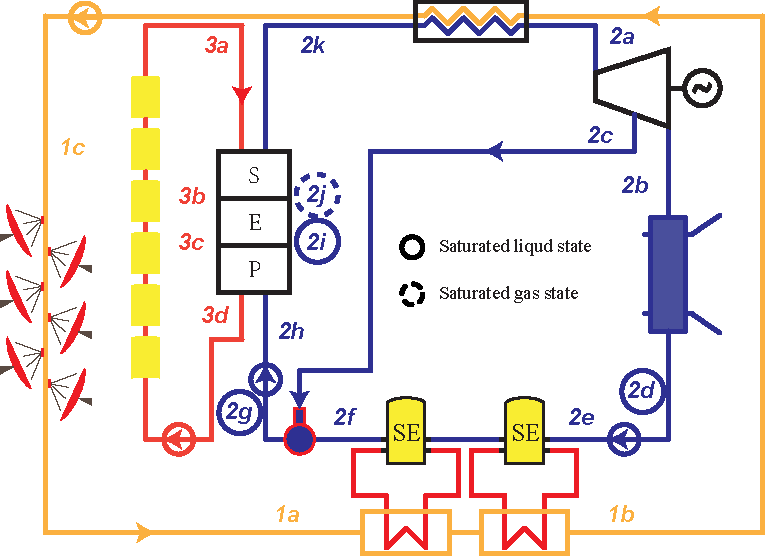
\includegraphics[width = 0.8\columnwidth]{fig/cascadeSystem}
	\caption{梯级系统结构示意图}
	\label{fig:System-1}
\end{center}
\end{figure}

梯级系统的水回路的$T$-$s$图如图\ref{fig:T-s_Water2}所示。在朗肯循环中,过程$2e$-$2f$的热量由斯特林机组提供。其传热过程曲线图如图\ref{fig:HeatTransfer_Water-SEs}所示。

\noindent \begin{figure}[htbp]
\centering
	\begin{subfigure}[b]{0.45\columnwidth}
	\includegraphics[width = \columnwidth]{fig/T-s_Water2}
	\caption{水循环的$T$-$s$图}\label{fig:T-s_Water2}
	\end{subfigure}
	~
\begin{subfigure}[b]{0.45\columnwidth}
	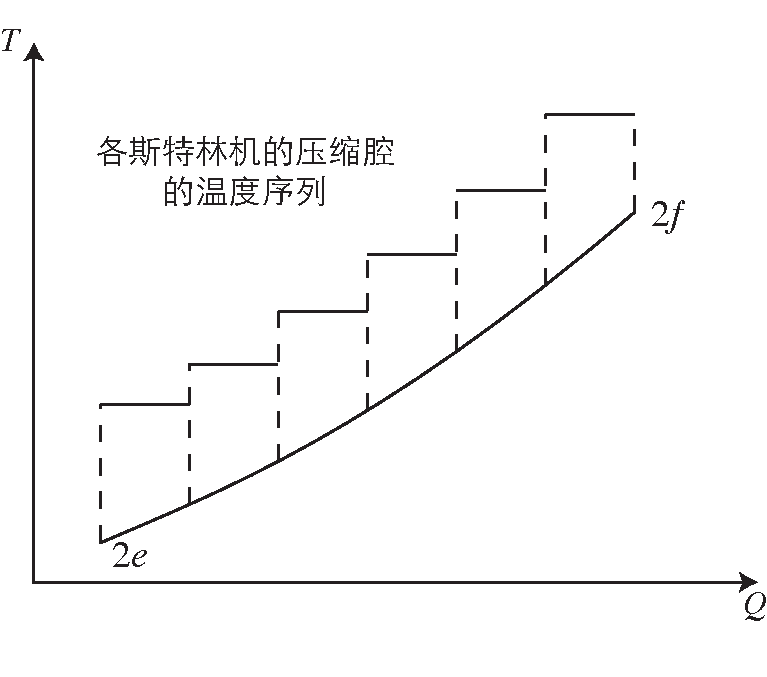
\includegraphics[width = \columnwidth]{fig/HeatTransfer_Water-SEs}
	\caption{$2e$-$2f$的传热过程曲线图}
	\label{fig:HeatTransfer_Water-SEs}
	\end{subfigure}
	
	\caption{水循环的过程曲线图和过程$2e$-$2f$的传热曲线图}\label{fig:Diagrams$2e$-$2f$}
\end{figure}


%\noindent \begin{figure}[htbp]
%\begin{center}
%	\subfigure[$T$-$s$ diagram of the water circuit]{
%	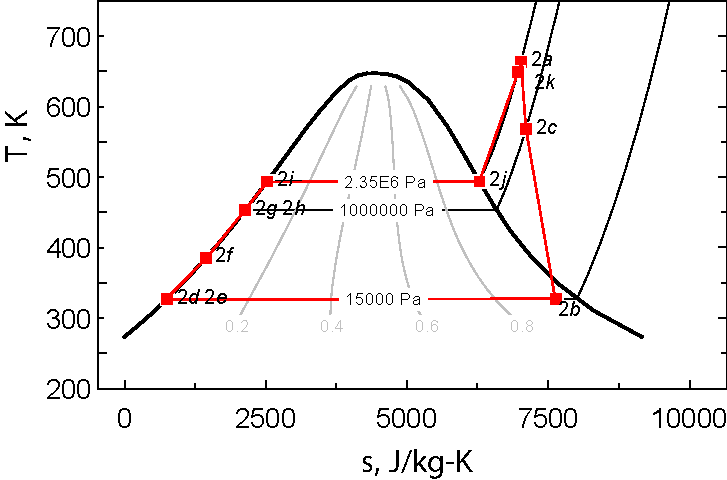
\includegraphics[width = 0.4\columnwidth]{fig/T-s_Water}
%	\caption{$T-s$ diagram of the water circuit}
%	\label{fig:T-s_Water}}
%	~\subfigure[Heat transfer diagram of process $2e$-$2f$]{
%	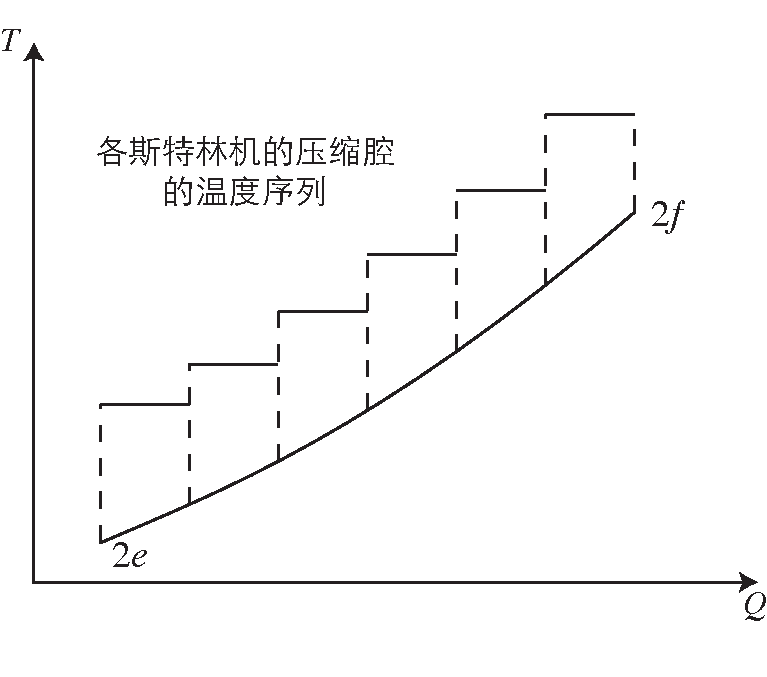
\includegraphics[width = 0.4\columnwidth]{fig/HeatTransfer_Water-SEs}
%	\caption{Heat transfer diagram of process $2e$-$2f$}
%	\label{fig:HeatTransfer_Water-SEs}}
%	\caption{Diagrams of water circuit and $2e$-$2f$ process}
%\end{center}
%\end{figure}

%\noindent \begin{figure}[htbp]
%\begin{center}
%	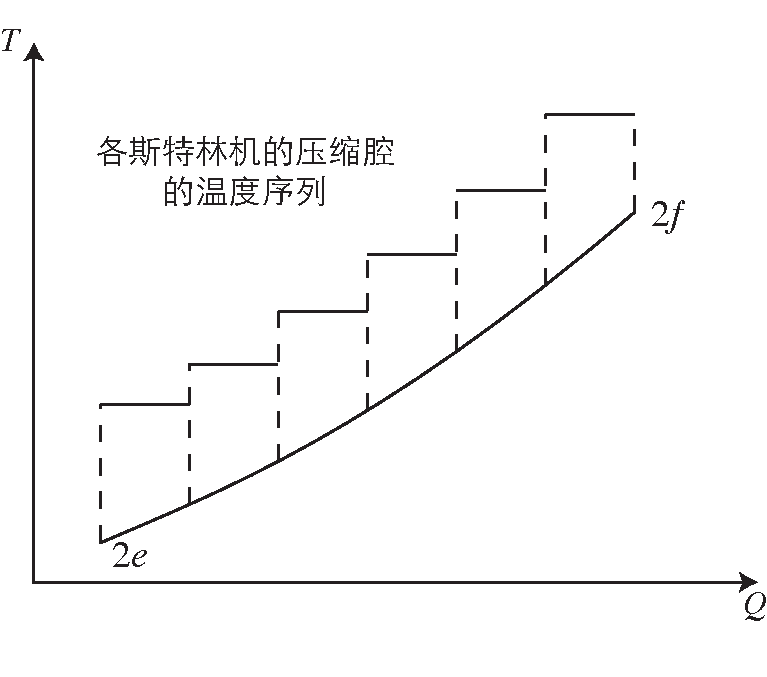
\includegraphics[width = 0.7\columnwidth]{fig/HeatTransfer_Water-SEs}
%	\caption{Heat transfer diagram of process $2e$-$2f$}
%	\label{fig:HeatTransfer_Water-SEs}
%\end{center}
%\end{figure}

%To build the cascade system model, several simplifying assumptions are made:
%
%\begin{itemize}
%	\item Steady state at nominal load of the system is analyzed.
%	\item Pressure drop due to flow is negligible.
%	\item The leak of working fluid in the pipes is neglected.
%	\item Same isentropic efficiency of steam turbine with different loads and in different stages.
%	\item Heat loss that occurs from the tube to the atmosphere is not considered.
%	\item There is no heat loss to the environment for Stirling engines.
%	\item Simple models are used of some processes and equipment.
%	\item A symmetrical regenerator behavior is assumed so that a single effectiveness can be defined as $e = (T_R - T_L) /(T_H - T_L)$.~\cite{Formosa2010, Juhasz2010}
%	\item A linear temperature profile across the regenerator exists, the mean effective temperature $T_{R} = (T_H-T_L) / \ln(T_H/T_L)$.~\cite{Der2007, Cavazzuti2012}
%\end{itemize}

\section{系统评估方法}
\subsection{系统性能}

梯级系统同时使用不同类型的集热器和不同种类的热力循环,它们相互耦合在一起。无法评价某一种型式的集热器收集的能量所产生的电能。一个更加通用的方式是定义系统的整体效率。梯级系统的整体光电转换效率等于总的输出功除以总的输入太阳能。
%The cascade system uses different types of collectors and different kinds of thermodynamic cycles. They are closely linked together. It is unable to indicate the output power of one specific kind of collector. A common approach is to define the overall efficiency of the system. The overall solar-to-electric efficiency equals to the total output power divided by the total input solar energy.

\begin{equation}
	\eta_{cs}=\dfrac{P_{cs}}{I_rA_{cs}} = \dfrac{P_{rk}+ P_{sea}}{I_rA_{tc} + I_rA_{dc}}
\end{equation}
\nomenclature[S]{rk}{Rankine cycle}

其中,$P_{rk}$是朗肯循环的输出功率,$P_{sea}$是所有斯特林机的输出功率之和。

\begin{equation}
	P_{rk} = P_{tb} - P_{pu} / \eta_{ge}
\end{equation}

汽轮机的功率
\begin{equation}
  P_{tb}=\left(1-y\right)\dot{m}_{2}\left(h_{2a}-h_{2b}\right)+y\dot{m}_{2}\left(h_{2a}-h_{2c}\right)
\end{equation}

泵消耗的功率
\begin{equation}
	P_{pu}=\left(1-y\right)\dot{m}_{2}\left(h_{2e}-h_{2d}\right)+\dot{m}_{2}\left(h_{2h}-h_{2g}\right)
\end{equation}

依据能量守恒,斯特林机组的输出总功率等于单位时间内热流体的焓降减去热流体的焓升。
\begin{equation}
	P_{sea}=\dot{m_1}(h_{1,i,1} - h_{1,o,n_1}) - \dot{m_2}(h_{2,o,n_1} - h_{2,i,1})
\end{equation}

正如前文提到的,$\dfrac{P_{rk}}{I_rA_{tc}}$并不能表明槽式集热器的发电效率,$\dfrac{P_{sea}}{I_rA_{dc}}$也不能表示碟式集热器的效率。

\subsection{系统对比方案}

梯级系统评估的另一个重要方面是与现有太阳能光热发电技术进行对比分析。主要有以下几种对比方案:

\begin{enumerate}[label=(\arabic*)]
	\item 同槽式系统进行对比。 

	当选择与槽式系统进行对比时,梯级系统获取的效率提升难以辨别出是由于采用梯级系统带来的提升还是只是由于采用了碟式集热器和斯特林机组带来的提升。
	\item 同碟式系统对比。
	
	当选择与碟式系统进行对比时,梯级效率获得的成本的降低难以区分是由于采用梯级系统带来的降低还是只是由于采用了槽式集热器和朗肯循环带来的降低。
	\item 与多种系统同时对比。
	
	一种自然的想法是,尽可能选用和梯级系统中相同的部件。这意味,需要同时选择槽式系统和碟式系统作为对比的系统。这两个系统独立存在,不存在梯级利用的关系,称为独立系统。
	
	由于独立系统和梯级系统的不同,独立系统中的槽式集热器和汽轮机不可能同时和梯级系统中的相同。同样,独立系统中的碟式集热器和斯特林机不可能同时和梯级系统中的相同。
	
	如果以相同的汽轮机输出功和相同的斯特林机输出功作为选择独立系统的条件,独立系统将具有和梯级系统不同的槽式集热面积以及不同的碟式集热面积。然而,这将非常不利于未来对梯级系统进行经济性对比分析,因为槽式集热器单位面积的成本和碟式集热器单位面积的成本相差很大。
	
	一个更好的选择方案则是,以相同的槽式集热器和相同的碟式集热器作为选择独立系统的条件,这样可以利用发电设备的变工况运行来实现不更换设备就能满足发电要求。同时,由于输出都是电能,可以很方便地进行效率对比分析和经济对比分析。
	
\end{enumerate}

本文选用以相同的槽式集热器和相同的碟式集热器作为选择独立系统的条件,即独立系统具有和梯级系统相同的槽式集热器和碟式集热器。

\section{系统参数的确定}

为了研究梯级系统的性能及其影响因素,需要对系统进行建模仿真分析。第\ref{cha:Modeling}章详细介绍了系统的建模方法。完成系统建模后,另一项重要的任务就是确定系统的参数。

系统中的参数主要由以下部分确定:

\begin{enumerate}[label=(\arabic*)]

\item 环境

典型的环境参数值设定为:
$I_r = 700\,\mathrm{W/m^2}$,$T_{amb} = 293\,\mathrm{K}$,$p_{amb} = 1\times10^5\,\mathrm{Pa}$,$v_{amb} = 1\,\mathrm{m/s}$。

\item 汽轮机

汽轮机以青岛捷能汽轮机集团股份有限公司的N-6 2.35系列产品为设计模型。其额定参数为:$P = 6\,\mathrm{MW}$,$p_s = 2.35\,\mathrm{MPa}$,$T_s = 390\mathrm{^\circ C}$,$\dot{m} = 32.09\,\mathrm{t/h}$,$p_c = 0.015\,\mathrm{MPa}$,$s_{tb} = 3000\,\mathrm{rpm}$。
	
	已知主汽参数,其比焓和比熵可以通过物性参数插件CoolProp获得:$h_s = 3.2203\times10^6\,\mathrm{J/kg}$,$s_s = 7.0149\times10^3\,\mathrm{J/(kg\cdot K)}$。
	
	汽轮机的排汽焓:$h_{c} = h_{s} - \dfrac{P}{\dot{m}} = 2.5472\times10^6\,\mathrm{J/kg}$.
	
	已知排汽压力以及$s_{i,c} = s_s$,汽轮机的理想排汽焓值可以由CoolProp获得:$h_{i,c} = 2.2737\times10^6\mathrm{J/kg}$。
	
	所以,汽轮机的等熵效率
	$\eta_{i,tb} = \dfrac{h_s - h_c}{h_{s} - h_{i,c}} = 0.71$.
	
	考虑到应用于本文提出的梯级系统,汽轮机的设计参数选择值见表ref{tab:CascadeSystemParameters}。
		 
\item 槽式集热器

由于LUZ公司的LS-3型号的集热器的试验数据比较丰富,本文选用它作为槽式集热器。它的主要参数见表\ref{tab:TroughParameters}~\cite{Fernandez2010}。

\begin{table}[htbp]
	\caption{LS-3型槽式集热器的主要参数}
	\begin{center}
	\begin{tabular}{cccccc}
		\toprule
		参数		&	值	&	参数		&	值	&	参数		&	值\\
		\midrule
		$A_{pc}$		&	$570.2\,\mathrm{m^2}$	&	$w_{dc}$	&	$5.76\,\mathrm{m}$	&	$L_{dc}$	&	$99\,\mathrm{m}$\\
		$f$	&	$1.71\,\mathrm{m}$	&	$d_i$		&	$0.066\,\mathrm{m}$	&	$d_o$	&	$0.07\,\mathrm{m}$\\
		$d_{abs,i}$	&	$0.113\,\mathrm{m}$	&	$d_{abs,o}$	&	$0.115\,\mathrm{m}$	&	Rim angle	&	$80^\circ$\\
		$\epsilon$		&	$0.15$	&	$\eta_{peak}$	&	$0.77$	&	$\rho$	&	$0.94$\\
		$\tau$	&	$0.95$	&	
$\alpha$	&	$0.96$	&	$Fe$	&	$0.97$\\
		\bottomrule
	\end{tabular}
	\end{center}
	\label{tab:TroughParameters}
\end{table}
\nomenclature{$f$}{焦距, m}

\item 碟式集热器

碟式集热器的反射镜选用SES公司的产品,而碟式接收器采用自行设计。碟式集热器的反射镜参数和接收器参数见表\ref{tab:dc}。

\item 斯特林机

梯级系统所用的斯特林机和第{sec:StirlingEngineModel}节中分析的斯特林机相同,即GPU-3型斯特林机,其参数见表{tab:GPU3parameters}。

\item 预热器

水在预热器中由过冷水被加热成饱和液态水,水在预热器的出口干度为0($x = 0$)。

此外,考虑到夹点温度,预热器的入口油温要比出口水温高出$\Delta T_{min}$,即$T_{3c} - T_{2i} = \Delta T_{min}$,$\Delta T_{min}$设定为$15\,\mathrm{K}$。

\item 蒸发器

水在蒸发器中由饱和液态水被加热成饱和蒸汽,水在蒸发器的出口干度为1($x = 1$)。

\item 过热器

过热器的入口油温受限于导热油的属性。在梯级系统中,导热油选用Therminol VP-1型合成油。它的物性参数可以通过CoolProp得到。过热器的入口油温设定为$T_{3a} = 623\,\mathrm{K}$。

\item 除氧器

除氧器具有两股入口流体和一股出口流体,它们都具有相同的压力。设定除氧器的压力$p_{se} = 1\times10^6\,\mathrm{Pa}$。除氧器的出口流体为饱和液态水,其干度为0($x = 0$)。

\item 空气-水换热器

空气-水换热器的入口空气温度设定为 $T_{1b} = 673\,\mathrm{K}$。
\end{enumerate}

\subsection{主要设计参数小结}
梯级系统的主要设计参数归纳见表\ref{tab:CascadeSystemParameters}。

\begin{table}[htbp]
	\caption{梯级系统的基本设计参数}
	\begin{center}
	\begin{tabular}{cccccc}
		\toprule
		参数		&	值	&	参数		&	值	&	参数		&	值\\
		\midrule
		$I_r$		&	$700\,\mathrm{W/m^2}$	&	$T_{dc,o}$	&	$1073\,\mathrm{K}$	&	$n_{se}$	&	100\\
		$T_{amb}$	&	$293\,\mathrm{K}$	&	$p_{dc}$		&	$5\times10^5\,\mathrm{Pa}$	&	$T_s$	&	$613\,\mathrm{K}$\\
		$p_{amb}$	&	$1\times10^5\,\mathrm{Pa}$	&	$\Delta{}T_{3,2,min}$	&	$15\,\mathrm{K}$	&	$p_s$	&	$2.35\times10^6\,\mathrm{Pa}$\\
		$v_{amb}$	&	$1\,\mathrm{m/s}$	&	$T_{tc,o}$	&	$623\,\mathrm{K}$	&	$p_c$	&	$1.5\times10^4\,\mathrm{Pa}$\\
		$P_{ge}$	&	$6\times10^6\,\mathrm{W}$	&	
$p_{tc}$	&	$2\times10^6\,\mathrm{Pa}$	&	$T_{s,d}$	&	$663\,\mathrm{K}$\\
		$T_{dc,i}$		&	$623\,\mathrm{K}$	&	$T_{1b}$	&	$673\,\mathrm{K}$	&	$p_{de}$ 	& 	$1\times10^6\,\mathrm{Pa}$\\			
		\bottomrule
	\end{tabular}
	\end{center}
	\label{tab:CascadeSystemParameters}
\end{table}

\section{对比系统的选择}

\noindent \begin{figure}[htbp]
\centering
	\begin{subfigure}[b]{0.64\columnwidth}
	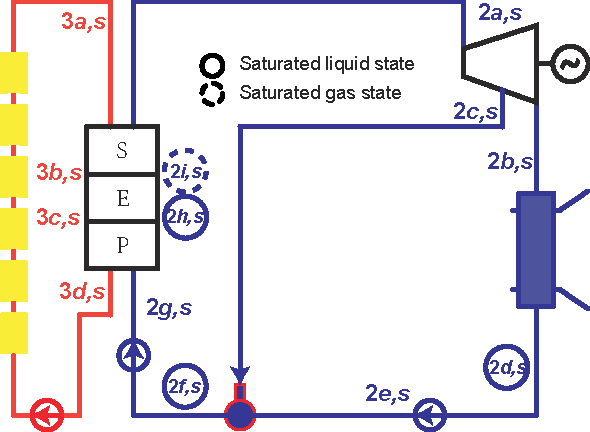
\includegraphics[width = \columnwidth]{fig/Trough-s}
	\caption{槽式-朗肯循环系统}\label{fig:TroughRankine}
	\end{subfigure}
	~
\begin{subfigure}[b]{0.26\columnwidth}
	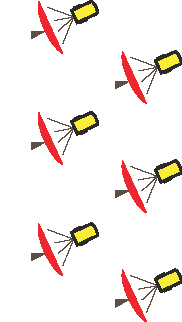
\includegraphics[width = \columnwidth]{fig/Dish-s}
	\caption{碟式-斯特林机系统}\label{fig:DishStirling}
	\end{subfigure}
	
	\caption{独立系统的结构示意图}\label{fig:Stand-alone-systems}
\end{figure}

%\noindent \begin{figure}[htbp]
%\begin{center}
%	\subfigure[Trough-Rankine system]{
%	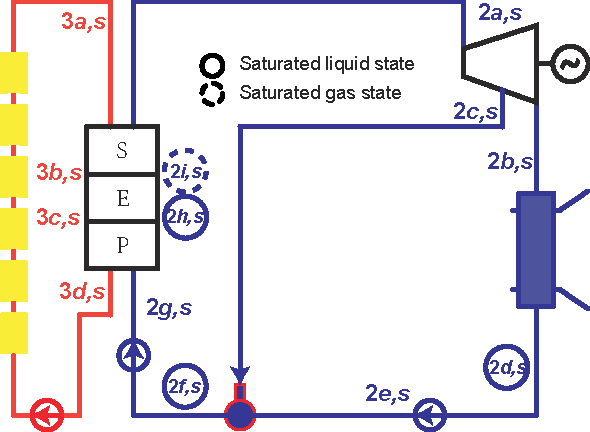
\includegraphics[width = 0.45\columnwidth, angle = 0]{fig/Trough-s}}
%	\subfigure[Dish-Stirling system]{
%	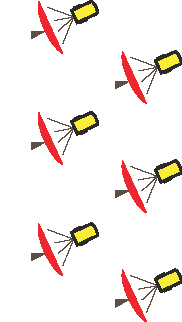
\includegraphics[width = 0.19\columnwidth, angle = 0]{fig/Dish-s}}
%	\caption{Sketch of the stand-alone systems}
%	\label{fig:Stand-alone-systems}
%\end{center}
%\end{figure}

Figure~\ref{fig:Stand-alone-systems} shows the sketch of the stand-alone systems. These two stand-alone systems are developed for comparison. They use the same dish collectors and trough collectors with the same thermal efficiencies of the cascade system.

\subsection{Stand-alone trough-Rankine system}

Steam turbine has the same main parameters and isentropic efficiency with that of the cascade system. Working pressure of deaerator is the same of the cascade system. So parameters of state $2b,s$ and $2c,s$ in Figure~\ref{fig:Stand-alone-systems} of the steam turbine can be expressed by
\nomenclature[S]{$s$}{Stand-alone systems}

\begin{equation}
	\eta_{i,tb}= (h_{2a,s}-h_{2b,s})/(h_{2a,s}-h_{i,2b,s}) = (h_{2a,s}-h_{2c,s})/(h_{2a,s}-h_{i,2c,s})
\end{equation}

The output power of steam turbine

\begin{equation}
	P_{tb,s}=\left(1-y_{s}\right)\dot{m}_{2,s}\left(h_{2a,s}-h_{2b,s}\right)+y_{s}\dot{m}_{2,s}\left(h_{2a,s}-h_{2c,s}\right)
\end{equation}

The output power of generator

\begin{equation}
	P_{ge,s}=P_{tb,s}\eta_{ge}
\end{equation}

The total power of pumps
\begin{equation}
	P_{pu,s}=\left(1-y_{s}\right)\dot{m}_{2,s}\left(h_{2e,s}-h_{2d,s}\right)+\dot{m}_{2,s}\left(h_{2g,s}-h_{2f,s}\right)
\end{equation}

Heat injected in the water circuit

\begin{equation}
	Q_{2,s}=\dot{m}_{2,s}\left(h_{2a,s}-h_{2g,s}\right)
\end{equation}

The generator efficiency is the same of that in the cascade system, and the efficiency of Rankine cycle can be expressed as

\begin{equation}
	\eta_{rk,s}=(P_{tb,s}-P_{pu,s}/\eta_{ge})/Q_{2,s}
\end{equation}

\subsection{Stand-alone dish-Stirling system}

In the stand-alone dish-Stirling system, Stirling engines with the same number of dish collectors are directly put on the focuses of the dish collectors. Water is used for cooling the Stirling engines. $T_{H,s}$ is chosen to be equal to outlet temperature of air in dish receiver. $T_{L,s}$ is chosen to be 310 K, the default expansion temperature in Fraser's dissertation~\cite{Fraser2008} for the calculation of 4-95 NK\uppercase\expandafter{\romannumeral2} engine. $k$ and $\gamma$ are chosen the same value as that of the Stirling engines in the cascade system.

\begin{equation}
	\eta_{sea,s}=\dfrac{T_{H,s}-T_{L,s}}{T_{H,s}+\dfrac{1-e_{s}}{k-1}\cdot\dfrac{T_{H,s}-T_{L,s}}{\ln\gamma}}
\end{equation}

where, $T_{R,s}=\dfrac{T_{H,s}-T_{L,s}}{\ln(T_{H,s}/T_{L,s})}$ and $e_{s}=\dfrac{T_{R,s}-T_{L,s}}{T_{H,s}-T_{L,s}}$.

The total power of Stirling engines

\begin{equation}
	P_{sea,s}=n_{dc}A_{dc}I_r\eta_{dc}\eta_{sea,s}
\end{equation}
\nomenclature{$n$}{Number of collectors}

\section{同独立系统的对比分析}
The results presented in Table~\ref{tab:importantResults} are issued using design parameters with counterflow of two fluids in Stirling engine array as the default flow type. It is shown that the cascade system with design parameters can achieve higher efficiency compared to corresponding stand-alone systems. Although the efficiency of the Stirling engine array is lower, the efficiency of the Rankine cycle is higher. The overall output power of the cascade system is $3.83\times10^4\,\mathrm{W}$ higher.
%Different results between two flow types of Stirling engine array are listed in Table~\ref{tab:SEAresults}.

\begin{table}[htbp]
	\caption{Some important results using design parameters}
	\begin{center}
	\begin{tabular}{cccccc}
		\toprule
		Parameter		&	Value	&	Parameter		&	Value	&	Parameter		&	Value\\
		\midrule
		$\eta_{cs}$		&	0.1974	&	$\eta_{sea,s}$	&	0.3786	&	$P_{ge,s}$	&	$5.826\times10^6\,\mathrm{W}$\\
		$\eta_{s}$	&	0.1962	&	$\eta_{rk}$	&	0.2660	&	$P_{sea}$		&	$3.552\times10^5\,\mathrm{W}$\\
		$\eta_{diff}$		&	0.0062	&	$\eta_{rk,s}$	&	0.2678	&	$P_{sea,s}$	&	$4.909\times10^5\,\mathrm{W}$\\
		$\eta_{sea}$	&	0.3407	&	$P_{ge}$		&	$6\times10^6\,\mathrm{W}$	&	$P_{diff}$		&	$3.830\times10^4\,\mathrm{W}$\\
		\bottomrule
	\end{tabular}
	\end{center}
	\label{tab:importantResults}
\end{table}
\nomenclature[S]{$cs$}{Cascade system}
\nomenclature[S]{$se$}{Stirling engine}
\nomenclature[G]{$\eta_{diff}$}{Efficiency difference of cascade system and stand-alone systems, $\eta_{cs}-\eta_{s}$}
\nomenclature[S]{$sea$}{Stirling engine array}
%\nomenclature{$P_{sea,s}$}{Total power of Stirling engines in stand-alone dish system, W}

\subsection{Effects of $I_{r}$}
\label{sec:I_r}

It is found that $I_r$ can affect the efficiency difference of cascade system and stand-alone systems $\eta_{diff}$. Figure~\ref{fig:I_r-eta_diff} shows curve fits of efficiency differences $\eta_{diff}$ versus $I_r$ with a series of different Stirling engine array power ratios. As it can be seen, for a high $I_r$ ($I_r > 550\,\mathrm{W/m^2}$), $\eta_{diff}>0$, the cascade system can achieve a higher efficiency than corresponding stand-alone systems. For a low $I_r$ ($I_r < 550\,$W/m$^2$), $\eta_{diff}$ may be negative. At this situation, the cascade system achieves a lower efficiency than corresponding stand-alone systems. This may be explained that instead of cooling water in the stand-alone dish-Stirling system, condensed water of Rankine cycle is used to cool the Stirling engines, which jeopardizes the heat dissipation and leads to a lower power of the Stirling engines. For a low $I_r$, the increased power of steam turbine due to absorbed heat by the condensed water is lower than the power loss of the Stirling engines. It can also be found that higher $I_r$ can achieve higher $\eta_{diff}$, which can be interpreted as the heat absorbed by the condensed water increases with $I_r$. So a higher $I_r$ location is always more suitable for cascade system. This means $I_r$ is a key factor to determine whether cascade system should be applied in a certain location.
\nomenclature[G]{$\beta$}{Ratio of power of Stirling engines to the total output power of cascade system}

\noindent \begin{figure}[htbp]
\begin{center}
	\includegraphics[width = 0.8\columnwidth, angle = 0]{fig/I_r-eta_diff}
	\caption{Curve fits of efficiency difference $\eta_{diff}$ versus $I_r$}
	\label{fig:I_r-eta_diff}
\end{center}
\end{figure}

\subsection{Effects of $\beta$}

As it can be seen in Table~\ref{tab:importantResults}, the $\eta_{diff}$ is very small with the design parameters given above. A reason $\eta_{diff}$ to be so small is that $\beta$, the ratio of power of Stirling engines to the total power, is very small, the heat released by the Stirling engine array is a small portion of the heat absorbed in the Rankine cycle. So increase $\beta$ may achieve higher $\eta_{diff}$. The relationship between $\eta_{diff}$ and $\beta$ under a series of $I_r$ is shown in Figure~\ref{fig:beta-eta_diff}. It can be found that, for a high $I_r$, increase $\beta$ may achieve a higher $\eta_{diff}$, but there is a limit. For $I_r=900$W/m$^2$, the maximum $\eta_{diff}=0.0228$ appears at $\beta=0.23$. For a low $I_r$, $\eta_{diff}$ is negative, increase $\beta$ will reduce $\eta_{diff}$. This can be explained as the same reason in Section~\ref{sec:I_r}.

\noindent \begin{figure}[H]
\begin{center}
	\includegraphics[width = 0.8\columnwidth, angle = 0]{fig/beta-eta_diff}
	\caption{Curve fits of efficiency difference $\eta_{diff}$ versus $\beta$}
	\label{fig:beta-eta_diff}
\end{center}
\end{figure}

\subsection{Effects of flow type}

Flow type between heating and cooling streams can affect the efficiency of Stirling engine array. Parallel flow, compared to counterflow, leads to higher Stirling engine efficiency in the first columns of the array for lower cooling temperature, while lower Stirling engine efficiency in the last columns for higher cooling temperature. 

\begin{table}[htbp]
	\caption{Results of Stirling engine array with two different flow types}
	\begin{center}
	\begin{tabular}{ccccccccc}
		\toprule
		\multirow{3}{*}{$x$}	&	\multicolumn{4}{c}{Parallel flow}	&\multicolumn{4}{c}{Counterflow}\tabularnewline
		\cline{2-5}	\cline{6-9}
		&$T_{1,i}$&$T_{2,i}$&$P_{sea}$&$\eta_{sea}$&$T_{1,i}$&$T_{2,i}$&$P_{sea}$&$\eta_{sea}$\tabularnewline
		&K&K&W&-&K&K&W&-\tabularnewline
		\midrule
		1	&	1073.15	&	327.17	&	5000	&	0.3648	&	1073.15	&	348.09	&	4867	&	0.3601\\
		2	&	1022.38	&	329.80	&	4630	&	0.3599	&	1023.25	&	345.48	&	4541	&	0.3562\\
		3	&	974.35	&	332.29	&	4280	&	0.3544	&	975.82	&	343.00	&	4230	&	0.3520\\
		4	&	928.90	&	334.65	&	3949	&	0.3485	&	930.75	&	340.65	&	3934	&	0.3474\\
		5	&	885.91	&	336.88	&	3635	&	0.3419	&	887.94	&	338.42	&	3654	&	0.3424\\
		6	&	845.26	&	339.00	&	3338	&	0.3347	&	847.28	&	336.29	&	3387	&	0.3370\\
		7	&	806.82	&	341.00	&	3057	&	0.3269	&	808.69	&	334.28	&	3134	&	0.3312\\
		8	&	770.49	&	342.91	&	2792	&	0.3184	&	772.06	&	332.37	&	2894	&	0.3248\\
		9	&	736.16	&	344.71	&	2541	&	0.3090	&	737.31	&	330.55	&	2666	&	0.3180\\
		10	&	703.75	&	346.43	&	2304	&	0.2989	&	704.37	&	328.82	&	2450	&	0.3106\\
		\bottomrule
	\end{tabular}
	\end{center}
	\label{tab:SEAresults}
\end{table}

Table~\ref{tab:SEAresults} shows the different results of the two flow types. The fit curves of temperature series of the heating and cooling fluids and the efficiency of Stirling engines in different columns are shown in Figure~\ref{fig:Parallelflow}
and~\ref{fig:Counterflow}.

%\noindent \begin{figure}[htbp]
%\begin{center}
%	\subfigure[Parallel flow]{
%	\includegraphics[width = 0.45\columnwidth, angle = 0]{fig/Parallelflow}}
%	\subfigure[Counterflow]{
%	\includegraphics[width = 0.45\columnwidth, angle = 0]{fig/Counterflow}}
%	\caption{Temperature series of two fluids and efficiency of Stirling engines in column $x$}
%	\label{fig:ParallelflowAndCounterflow}
%\end{center}
%\end{figure}

\noindent \begin{figure}[htbp]
\begin{center}
	\includegraphics[width = 0.8\columnwidth, angle = 0]{fig/Parallelflow}
	\caption{Parallel flow: Temperature series of two fluids and efficiency of Stirling engines in column $x$}
	\label{fig:Parallelflow}
\end{center}
\end{figure}
\noindent \begin{figure}[H]
\begin{center}
	\includegraphics[width = 0.8\columnwidth, angle = 0]{fig/Counterflow}
	\caption{Counterflow: Temperature series of two fluids and efficiency of Stirling engines in column $x$}
	\label{fig:Counterflow}
\end{center}
\end{figure}

It can be concluded that the temperature increment of cooling fluid is much smaller than the temperature decrement of heating fluid due to their large difference of $c_p\dot{m}$, which leads to a small difference of overall efficiency of Stirling engine array between the two flow types.

To find out a clear difference of the two flow types, a simple model of Stirling engine array is developed with air as the heating fluid and water as the cooling fluid. $T_{1,i}, T_{1,o}, T_{2,i}, q_{1,m}$ are fixed and chosen the same values as in the cascade system. Change the value of $q_{2,m}$, and the corresponding Stirling engine array efficiency of the two flow types ($\eta_p$ and $\eta_c$) can be obtained. Figure~\ref{fig:SEAflowtypes} shows the efficiency of Stirling engine array with different $q_{2,m}$ in two flow types. It can be found that counterflow has a higher efficiency than parallel flow, and with lower $q_{2,m}$ comes with higher efficiency difference.
\nomenclature[S]{$p$}{Parallel flow; particular solution; piston}
%\nomenclature[S]{$c$}{Counterflow}

For a system with large difference of $c_p\dot{m}$ of two fluids, that means one fluid can only achieve a small temperature rise (drop) compared to the other fluid, will lead to a small difference of two flow types. For a system with similar difference of $c_p\dot{m}$, use the counterflow can achieve a higher efficiency.

\noindent \begin{figure}[H]
\begin{center}
	\includegraphics[width = 0.8\columnwidth, angle = 0]{fig/SEAflowtypes}
	\caption{Efficiency of Stirling engine array with different $q_{2,m}$}
	\label{fig:SEAflowtypes}
\end{center}
\end{figure}
%\section{System evaluation}

\section{本章小结}

In this chapter, an effective typical cascade system proposed in Chapter~\ref{cha:SystemTopology} is chosen for evaluation. 
This cascade system uses two different types of collectors and two different power generation methods. 
Steam Rankine cycle is applied for this system for its widely applied applications.
Reasonable parameters are selected and the system model is developed.
Two stand-alone systems are chosen as the comparison systems for system evaluation. 
They use the same dish collectors and trough collectors of the cascade system. 
Simulations of the cascade system are carried out and results are compared with corresponding stand-alone systems.

Results show that $I_r$ is the key factor to determine whether cascade system should be applied in a certain location. Compared to corresponding stand-alone systems, the cascade system can achieve a higher efficiency with high solar irradiance ($I_r > 550\,\mathrm{W/m^2}$). The directions to increase the efficiency difference between cascade system and corresponding stand-alone systems are also considered. To design a cascade system including Stirling engine array, flow type of fluids for heating and cooling Stirling engine array is also required to be considered. 

%However, it has to be pointed out that this thesis uses a simple Stirling cycle efficiency formula given in the book~\cite{Stine1985}. This formula takes no consideration of various losses and irreversibilities, such as pressure drop, shuttle conduction, finite speed of piston and mechanical friction. The heat transfer process between the fluids and the Stirling engines has been simplified to be constant heat transfer coefficient. However, the imperfect model of the Stirling engine doesn't affect the idea of solar thermal cascade system presented in this thesis. More accurate Stirling engine model can be applied to achieve higher accuracy of the system in the future work. Besides, a cascade system with a different $\beta$ not only affects the efficiency of the system but also changes the portion of dish collector area to the total collector area, which will affect the cost. The cost analysis and optimization research of the cascade system is not included in this thesis, which are worthy candidates for further research.